\chapter{Introduction aux courbes elliptiques}
\section{Généralités}
\subsection{Définitions}
\begin{definition}
Une équation de Weierstrass affine généralisée d'une courbe elliptique $E$ sur \field{} est donnée par :
\begin{equation}
y^2 + a_1 xy + a_3 y = x_3 + a_2x^2 + a_4x + a_6
\end{equation}
\begin{equation}
f(x, y) = y^2 + a_1 xy + a_3 y - x_3 - a_2x^2 - a_4x - a_6
\end{equation}
avec $a_1, a_2, a_3, a_4, a_5, a_6  \in \field{}$ et $\Delta \neq 0$ où $\Delta$ est le discriminant de $E$ et est défini de la façon suivante : 
\begin{equation}
\begin{cases}
\Delta & = -b_2^2 b_8 - 8b_4^3 - 27b_6^2 + 9 b_2b_4b_6\\
b_2 &= a_1^2 + 4a_2,\\
b_4 &= 2a_4 + a_1a_3\\
b_8 &= a_1^2a_6 + 4a_2a_6 - a_1a_3a_4 + a_2a_3^2 - a_4^2
\end{cases}
\end{equation}
\end{definition}

\vspace{0.5cm}

\begin{itemize}[label=--]
    \item Une courbe elliptique consiste à l'ensemble des zéros d'un polynôme à deux variables de degré trois de la forme précédente auquel on adjoint un point à l'infini. C'est donc une courbe plane algébrique.
    \item La condition $\Delta \neq 0$ assure (et réciproquement) que la courbe $E$ ne possède aucun points singuliers à coordonnées dans \closure{} \footnote{Les coordonnées des points sont automatiquement algébriques.}, c'est à dire de points dont les dérivées partielles s'annulent. Si $f(x_1, y_1) = 0$ avec $(x_1, y_1) \in \closure{}^2$, alors le vecteur $\left (\frac{\delta P}{\delta x}(x_1, y_1), \frac{\delta P}{\delta y}(x_1, y_1) \right )$ n'est pas le vecteur nul. On parle alors de courbe \emph{non singulière} ou \emph{lisse}. Cette équivalence se vérifie sans peine. 
    \item Un point de la courbe est non singulier s'il admet une unique tangente en ce point. Cela se traduit par l'absence de racines multiples\footnote{La nullité du discriminant d'un polynôme équivaut à la présence de racines multiples dans son corps de décomposition.}. La figure \ref{fig:EC} représente les graphes de courbes elliptique à valeurs dans différents corps.
\end{itemize}

\begin{definition}
Soit $\field{} \hookrightarrow \field[L]$ une extension de corps. Il est possible de s'intéresser à l'ensemble des points de la courbe $E/\field{}$ dans n'importe quelle extension algébrique de \field{}. On parle des points \field[L]-rationnels de $E/\field{}$. Lorsque rien n'est précisé, on considère implicitement la clôture algébrique de $\closure{}$, $E(\closure{})$.
\begin{equation}
    E(\field[L]) = \{(x,y) \in \field[L]^2\ \mid\ f(x,y) = 0\} \cup \{O\}
\end{equation}
Le corps \field[L] est appelé \emph{corps des points rationnels}\footnote{Ground field.}. Qu'il ne faut pas confondre avec le corps de base\footnote{Base Field.} \field{} qui est le plus petit corps contenant les coefficients de l'équation.
\end{definition}

\begin{figure}[ht]
\centering
    \subfigure[Courbes elliptiques sur \R]
    {
       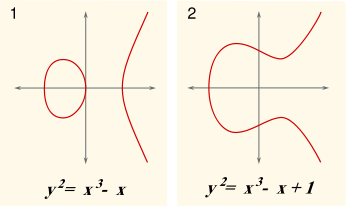
\includegraphics[scale=0.6]{images/EC_R.png}
       \label{fig:ECR}
     }
     \subfigure[Courbe elliptique sur un corps fini]
     {
       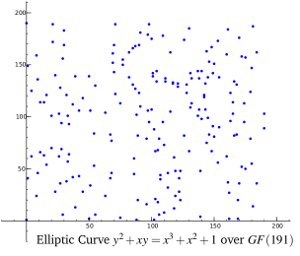
\includegraphics[scale=0.5]{images/EC_ff.png}
       \label{fig:ECFF}
     }
    \label{fig:EC}
    \caption{Graph de courbes elliptiques}
\end{figure}

\vspace{0.5cm}
Quelques rappels sur l'\emph{espace projectif} s'impose. C'est une construction qui permet d'homogénéiser un espace vectoriel, autrement dit d'oublier les proportionnalités pour ne plus considérer que les directions.
\begin{definition}
Soit $E$ un \field{}-espace vectoriel. L'\emph{espace projectif} déduit de $E$ et noté \ensnombre{P}$(E)$  est l'ensemble des droites vectorielles de $E$.

En d'autres termes, si $\mathcal{R}$ est la relation d'équivalence \og être proportionnel \fg{} sur $E\backslash \{0\}$ définie par $x\mathcal{R}y$ si et seulement si il existe $\lambda \in \field{}^*$ tel que $x = \lambda y$, alors $\ensnombre{P}(E) = (E \backslash \{0\}) /_{\mathcal{R}}$.

Une classe d'équivalence, noté $[X_1 : \ldots : X_n]$, est appelé \emph{coordonnée homogène}. Chacune de ces classes correspond à une droite vectorielle privée de zéro. Par définition, pour tout $\lambda \in \field{}^*$, $[X_1 : \ldots : X_n] = [\lambda X_1 : \ldots : \lambda X_n]$.

Les points tels que $X_n = 0$ sont appelés \emph{points à l'infini}.

Si $E = \field{}^n$, on note \ensnombre{P}$(E) = \ensnombre{P}^n(\field{})$, l'espace projectif de dimension $n$. $\ensnombre{P}^1(\field{})$ est la droite projective et $\ensnombre{P}^2(\field{})$ est le plan projectif.

$\ensnombre{P}^n(\field{}) \simeq \ensnombre{A}^n(\field{}) \times \ensnombre{P}^{n-1}(\field{})$
\end{definition}

Citons deux articles intéressant du site Images des Mathématiques sur l'espace projectif : \href{http://images.math.cnrs.fr/L-infini-est-une-droite-comme-les.html}{Art 1}, \href{http://images.math.cnrs.fr/Et-si-on-rajoutait-une-droite-a-l.html}{Art 2}.

\begin{figure}[ht]
    \centering
    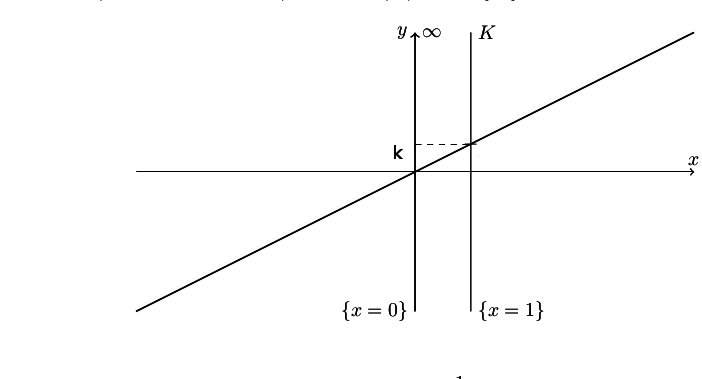
\includegraphics[scale=0.4]{images/projectif.png}
    \caption{La droite projective s'identifie à l'espace affine de dimension un auquel on ajoute un point à l'infini}
    \label{fig:projectif}
\end{figure}

\begin{definition}
Une équation de Weierstrass généralisée projective d'une courbe elliptique $E$ sur un corps \field{} est donnée par :
\begin{equation}
E : Y^2Z + a_1XYZ + a_3YZ^2 = X^3 + a_2X^2Z + a_4XZ^2 + a_6Z^3
\end{equation}
avec $a_1, a_2, a_3, a_4, a_5, a_6  \in \field{}$ et $\Delta \neq 0$.
\end{definition}

\begin{itemize}[label = --]
    \item Soit $f(x,y) = 0$ une courbe affine. On obtient sa version projective en définissant la courbe $\tilde{f}(x,y,z) = 0$ où $\tilde{f}$ est le polynôme homogène associé à $f$. $\tilde{f}(x,y,z) = z^n f(x,y)$ et $\tilde{f}(x,y,1) = f(x,y)$.
    \item Le point à l'infini, noté \infini{}, correspond à $[0 : 1 : 0]$.
    \item On peut montrer que le point à l'infini est non singulier.
\end{itemize}

\vspace{0.3cm}

Nous n'avons pas pour le moment défini ce qu'est une courbe elliptique. Nous nous sommes contentés de donner une équation de cet objet. L'équation de Weierstrass est une incarnation possible d'une courbe elliptique. Mais il en existe d'autre que nous verrons ultérieurement (forme de Legendre, forme Hessienne \ldots ). L'équivalence des définitions se démontrent à l'aide du théorème de Riemann-Roch.

\begin{definition}
Une courbe elliptique $E$ sur un corps \field{} est une courbe algébrique projective non singulière de genre $1$ avec la donnée d'un point \field{}-rationnel \infini{}.
\end{definition}

\subsection{Isomorphismes}
Finalement la donnée d'une courbe elliptique correspond à la donnée du corps de base \field{} et des coefficients $a_1, \ldots, a_6$ régissant son équation de Weierstrass. C'est ce qu'on appelle les \emph{paramètres}\footnote{Domain parameter.} d'une courbe elliptique. Dans le cadre de la cryptographie, on ajoute aussi le point de base $P$, l'ordre $l$ de ce point, ainsi que le cofacteur $h$. 

Tout d'abord, remarquons que via un changement de variables adapté et qu'en fonction de la caractéristique du corps, il est possible d'obtenir une équation de Weierstrass réduite. Par exemple, si la caractéristique du corps \field{} est différente de $2$ alors on peut simplifier l'équation en complétant le carré de gauche : $y \mapsto y + a_1x/2 + a_3 /2$. De la même manière, lorsque la caractéristique du corps de base est différente de $3$, on peut éliminer le coefficient $a_4$ via : $x \mapsto x + a_2/3$. Le tableau \ref{tab:weierstrass} résume la situation. En particulier lorsque $char(\field{}) \neq 2, 3$, on obtient une équation appelée \emph{équation Weierstrass simplifiée}\footnote{Short Weierstrass Form.}.
\begin{comment}
\begin{figure}[h]
\centering
    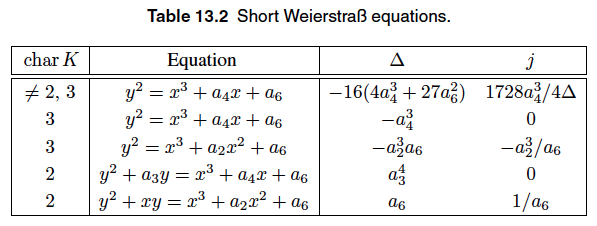
\includegraphics[scale=0.5]{images/equationWeierstrass.png}
    \caption{Equation de Weierstrass}
    \label{fig:weierstrass}
\end{figure}
\end{comment}

\begin{table}[ht]
\centering
\begin{tabular}{|c|c|cc|}
\hline
char \field{} & Equation & $\Delta$ & $j$  \\
\hline \hline
\rule[0ex]{0pt}{3ex}
$\neq 2, 3$ & $y^2 = x^3 + ax + b$ & $-16(4a^3 + 27b^2)$ & $1728 \ 4 a^3 / \Delta$\\
3 & $y^2 = x^3 + ax + b$ & $-a^3$ & 0 \\
3 & $y^2 = x^3 + a_2x^2 + a_6$ & $-a_2^3a_6$ & $-a_2^3/a_6$\\
2 & $y^2 + a_3y = x^3 + a_4x + a_6$ & $a_3^4$ & $0$ \\
2 & $y^2 + xy = x^3 + a_2x^2 + a_6$ & $a_6$ & $1/a_6$\\
\hline
\end{tabular}
\caption{\'Equation de Weierstrass en fonction de la caractéristique du corps}
\label{tab:weierstrass}
\end{table}

\todo{Comment calculer le discriminant ? }

Nous nous intéressons maintenant à la notion d'\emph{isomorphisme de courbes elliptiques}. Intuitivement un isomorphisme correspond à un renommage des éléments. Deux courbes elliptiques isomorphes sont semblables. Elles possèdent les mêmes propriétés. \'A un renommage près, ce sont exactement les mêmes courbes. Toutes les propriétés vraies pour l'une le sont aussi pour l'autre, la seule différence (du point de vue de la structure étudiée) réside dans le nom que l'on attribue aux différents points. C'est la raison pour laquelle on raisonne à isomorphisme près.

\begin{definition}
Deux courbes elliptiques $E_1, E_2$ sur \field{} sont isomorphes sur \field{} s'il existe $u, r, s, t \in \field{}$ et $u \ne 0$ tel que le changement de variables 
\begin{equation*}
    (x, y) \mapsto (u^2x + r, u^3y + u^2sx + t)
\end{equation*}
transforme l'équation de Weierstrass $E_1$ en l'équation de Weierstrass de $E_2$. C'est ce qu'on appelle un changement de variables admissibles. Cette transformation est réversible. Et son inverse définit un changement de variables admissibles de $E_2$ vers $E_1$. Un tel isomorphisme définit une bijection entre l'ensemble des points rationnels de $E_1$ et ceux de $E_2$.
%Remarquez que même si deux courbes sont isomorphes sur une extension de \field{}, la courbe isomorphe est bien définie dans le corps \field{}.
\end{definition}

Une isogénie de degré $1$ est un isomorphisme. Ainsi l'application précédente est bien un isomorphisme et un morphisme de groupe. On peut aussi le voir d'une autre façon. La loi de groupe est définie par le fait que les points $P, Q, R$ sont alignés si et seulement si $P + Q + R = \infini{}$. De plus dire que notre isomorphisme préserve la structure de groupe c'est dire exactement que si $P, Q, R$ sont alignés alors $\phi(P), \phi(Q), \phi(R)$ sont alignés. Ou en d'autres termes que l'image d'une droite est encore une droite. Or un changement de variables admissibles est une transformation affine et par définition elle envoie une droite sur une autre droite.

\vspace{0.2cm}

\begin{propriete}
Lorsque $char(\field{}) \geq 5$, alors deux courbes elliptiques $E_{(a, b)},\ E_{(a^{'}, b^{'})}$ sont isomorphes sur \field{} si et seulement si il existe $u \in \field{}^{*}$ tel que $(x, y) \mapsto (u^2x, u^3y)$ si et seulement si il existe $u \in \field{}^{*}$ tel que $a = u^4 a^{'}$ et $b = u^6 b^{'}$.
\end{propriete}

\begin{theoreme}
\^Etre isomorphe est une relation d'équivalence sur l'ensemble des courbes défini sur \GF{q}. Ce qui nous intéresse, n'est pas de savoir le nombre de courbes mais plutôt le nombre de classes d'isomorphisme (ie : le nombre de familles de courbes réellement distinctes)\footnote{Une classe d'isomorphisme contient un ensemble de courbes. Bien qu'elles possèdent chacune une équation qui leur est propre, structurellement elles sont identiques. Ce sont les mêmes courbes mais avec des noms différents.}. Le nombre de classes d'isomorphisme sur \GF{q} est $2q + 6$, $2q + 2$, $2q + 4$, $2q$ pour $ q \equiv 1, 5, 7, 11 \pmod{12}$.\begin{proof}
Au total il y a $q(q-1)$ courbes elliptiques (il faut que le discriminant soit non nul). Certaines courbes sont isomorphes entre elles. Trois cas disjoints sont à distinguer : $(a, 0)$, $(0, b)$ et $(a, b)$ avec dans chaque cas $a$ et $b$ non nuls. 
\begin{enumerate}
    \item $(a, 0)$ avec $a \neq 0$. Il existe $q-1$ courbes de cette forme. $Cl(a, 0) = \{ (u^4a, 0) \mid u \in \GF{q}^* \}$. Ainsi $\# Cl(a, 0) = (q-1)/(2 \text{ ou } 4)$. En fait, on a $\# Cl(a, 0) = (q-1)/ \# Aut(E)$.
    \item $(0, b)$ avec $b \neq 0$. Il existe $q-1$ courbes de cette forme. $Cl(0, b) = \{ (0, u^6 b) \mid u \in \GF{q}^* \}$. Ainsi $\# Cl(0, b) = (q-1)/(2 \text{ ou } 6)$.
    \item $(a, b)$ avec $ab \neq 0$. Il existe $(q-1)(q-2)$ courbes de cette forme. $Cl(a, b) = \{ (u^4a, u^6b) \mid u \in \GF{q}^* \}$. Ainsi $\# Cl(a, b) = (q-1)/2$.
\end{enumerate}
Finalement, le nombre de classes dépend de l'existence ou non d'un élément d'ordre $3$ (ie : si $3 \mid q-1$) et d'un élément d'ordre $4$ (ie : si $4 \mid q-1$ car $\GF{}^*$ est un groupe cyclique).
\end{proof}
Ce qu'il faut retenir est qu'il existe environ $2q$ courbes définies sur \GF{q} structurellement distinctes.
\end{theoreme}

\begin{propriete}
Supposons que $char(\field{}) \geq 5$. Soit $E$ une courbe elliptique définie sur \field{}.
\begin{itemize}[label=$\bullet$]
    \item Si $a_4 = 0$, alors pour tout $a_6^{'} \in \field{}^{'}$, la courbe $E$ est isomorphe à $y^2 = x^3 + a_6^{'}$ sur $\field{}((a_6/a_6^{'})^{1/6})$. C'est une extension de degré au plus 6. On parle de \emph{twist sextique}.
    \item Si $a_6 = 0$, alors pour tout $a_4^{'} \in \field{}^{'}$, la courbe $E$ est isomorphe à $y^2 = x^3 + a_4^{'}x$ sur $\field{}((a_4/a_4^{'})^{1/4})$. Extension de degré au plus 4. On parle de \emph{twist quartique}.
    \item Si $a_4a_6 \neq 0$, alors pour tout $v \in \field{}^{'}$, la courbe $E$ est isomorphe à $\tilde{E_v} : y^2 = x^3 + a_4v^2x + a_6v^3$ sur $\field{}(\sqrt{v})$. $\tilde{E_v}$ est elle-même isomorphe à $vy^2 = x^3 + ax + b$. On parle de \emph{twist quadratique} lorsque $v$ est un non résidu quadratique dans \field{}, ie : $\sqrt{v} \notin \field{}$.
\end{itemize}
Deux courbes elliptiques sont twist ou tordues l'une de l'autre si et seulement si elles ont le même j-invariant. On qualifie le twist de quadratique, quartique ou sextique afin de préciser le degré de l'extension dans lequel est défini l'isomorphisme. On parle du twist car il est unique à isomorphisme près.
Soit $E$ une courbe définie sur \GF{p}, on peut s'intéresser au twist de $E(\GF{p^k})$. Dans ce cas, on sélectionne $v \in \GF{p^k}^*$, le twist sera défini dans $\GF{p^k}$ et l'isomorphisme dans $\GF{p^k}(\sqrt{v})$. 
Par abus de langage, le twist fera souvent référence au twist quadratique.
\end{propriete}

\todo{Prouver que le twist est unique à isomorphisme près. Cf. Vitse mémoire M2.}

\begin{propriete}
La somme des points sur \GF{q} d'une courbe elliptique et de son twist quadratique est constant et vaut $2q + 2$.
\begin{equation}
\#E_{a, b}(\GF{q}) + \#\tilde{E_v}(\GF{q}) = 2q + 2
\end{equation}
\begin{equation}
\#E(\GF{q}) = q + 1 - t
\end{equation}
\begin{equation}
\#\tilde{E}(\GF{q}) = q + 1 + t
\end{equation}
Cette propriété est utile lorsque l'on recherche de bonne courbes elliptique pour la cryptographie. En effet on peut déterminer l'ordre de deux courbes elliptiques pour le prix d'un.
\end{propriete}
\begin{proof}
$E_{a, b} : y^2 = f(x)$ et $\tilde{E_v} : y^2 = f_v(x) = v^3 f(x/v)$. Lorsque $x$ parcourt \GF{q}, $x/v$ parcourt \GF{q}. \'Etant donné un élément $x$ quelconque de \GF{}, il suffit de distinguer les cas (disjoints) où $f_v(x)$ est nul, est un carré non nul et est un non carré dans \GF{q} afin de s'apercevoir qu'on obtient au total à chaque fois deux points distincts de la courbe $E$ ou (inclusif) de son twist. 
\end{proof}


\begin{theoreme}
Soit E une courbe elliptique définie sur \GF{q}, alors on a $\# E(\GF{q^n}) = q^n + 1 - t_n$, avec $t_n = \alpha^n + \overline{\alpha}^n$, $t_0 = 2, t_1 = t$ et $t_{n+1} = t*t_n - q*t_{n-1}$.
Ainsi on a : $t_{2n}(-t) = t_{2n}(t)$ et $t_{2n+1}(-t) = -t_{2n+1}(t)$.
Finalement deux courbes isomorphes sur \GF{q^d} ont le même cardinal sur \GF{q^d} mais sur les sous-corps ou les extensions de corps de \GF{q^d} ça n'est pas le cas en général \footnote{Pour les courbes de traces nulles, commes les courbes supersingulières sur un corps de caractéristique supérieur à $4$, ça n'est pas vrai, elles ont le même cardinal quelque soit le corps des points rationnels considérés.}. Par contre pour les extensions de degré pair de \GF{q^d}, elles ont le même cardinal.
Par exemple, soit $E_1$ le twist quadratique de $E_2(\GF{q})$. Alors on a $\# E_1(\GF{q^2}) = \# E_2(\GF{q^2})$ et même $\# E_1(\GF{q^{2n}}) = \# E_2(\GF{q^{2n}})$. Mais par contre elles n'ont pas, a priori le même cardinal sur leur corps de base puisque leurs traces sont opposées.
\end{theoreme}


La trace d'une courbe est égale à l'opposé de la trace de son twist. La courbe et son twist sont de même cardinal lorsque les points sont pris à valeur dans une extension de degré pair du corps de base. Pour les extensions impaires, le cardinal est identique pour les courbes supersingulières par exemple (car la trace est nulle).


Existe t-il un moyen simple de savoir si deux courbes elliptiques sont isomorphes sur un corps algébriquement clos ? 

\begin{propriete}
Deux modèles de Weierstrass simplifiés sont \closure{}-isomorphe si et seulement si ils ont le même j-invariant. Pour l'implication directe, un isomorphisme sur \field{} est suffisant. De plus étant donné $j_0 \in \field{}$, il existe un modèle de Weierstrass sur \field{} avec un j-invariant égal à $j_0$.

Ainsi si \field{} est algébriquement clos, les classes d'isomorphisme de courbes elliptiques sont en bijection avec les éléments de \field{} via l'application $E \mapsto j_E$.
\end{propriete}
\begin{itemize}[label=$\bullet$]
    %\item $E_1 \underset{\field{}}{\simeq} E_2 \Longleftrightarrow \exists u \in \field{}^{*}, a = u^4 a^{'}$ et $b = u^6 b^{'}$.
    \item $j(E_1) = j(E_2) \Longleftrightarrow a^3 b^{'2} = a^{'3}b^{2}$
    \item $j(E) = 0 \Longleftrightarrow a_4 = 0$ \hspace{1cm} $j(E) = 1728 \Longleftrightarrow a_6 = 0$
    \item Soit $j_0 \in \field{}, \neq 0, 1728$, notons $k = j / (1728 - j)$. Alors l'ensemble des courbes elliptique ayant leur j-invariant égal à $j_0$ sont de la forme $y^2 = x^3 + 3kcx + 2kc$ avec $c \in \field{}$. 
    %\item $j(E) \neq 0, 1728 \Longleftrightarrow$
    %\item Si $a_4 = 0$ 
\end{itemize}


\subsection{Loi de groupe}
L'ensemble des points d'une courbe elliptique peut être muni d'une structure de groupe abélien dont l'élément neutre est le point à l'infini. La loi de groupe peut être interprétée géométriquement grâce à la fameuse méthode des tangentes et des sécantes \footnote{Chord and tangent method.}.

\begin{figure}[ht]
\centering
    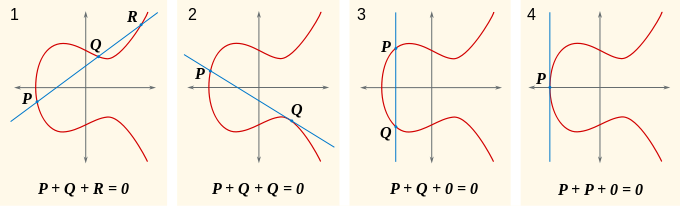
\includegraphics[scale=0.5]{images/EC_group.png}
    \caption{Loi de groupe}
    \label{fig:EC_group}
\end{figure}

\begin{itemize}[label=--]
    \item Lire Implicit differentiation pour le coefficient directeur d'une tangente.
    \item La seule difficulté consiste à prouver l'associativité et ce n'est pas facile. Dans un premier temps, on peut envisager une preuve directe par identification des formules. Mais il faut tenir compte des différentes exceptions. De plus elle s'avère être pratiquement infaisable à la main. On peut se servir de logiciels de calculs formels. Une preuve possible est de montrer qu'une courbe elliptique est isomorphe au groupe de Picard. \href{http://math.rice.edu/~friedl/papers/AAELLIPTIC.PDF}{Preuve élémentaire}.
    \item L'opposé est gratuit. Soit $P = (x, y)$, alors $-P = (x, -a_1x - a_3 - y)$. $-P = (x, -y)$ sur un corps premier et $-P = (x, x+y)$ sur un corps binaire. Cette propriété permet d'accélérer la ECSM via le recodage du scalaire.
    \item L'addition est indépendante des coefficients de la courbe et le doublement ne dépend que du coefficient $a$. Ainsi les formules restent valables pour les courbes vérifiant $a_2 = a$. Un attaquant peut transmettre un point d'une autre courbe de petit ordre. Si aucun test n'est réalisé, l'utilisateur calculera une ECSM sur une courbe faible sans se rendre compte de rien : \emph{Invalid Curve Attacks}. 
    \item De la même façon, on remarque que les formules en X-only (employées par les algorithmes d'échelle) s'appliquent indifféremment sur une courbe ou sur son twist (que se soit pour les courbes de Montgomery ou pour courbes de Weierstrass). Il convient donc de vérifier que les points reçus appartiennent bien à la courbe et non au twist ou bien sélectionner une courbe dont le twist est sécurisé (twist secure). Remarquez que le test peut-être contourné en injectant une faute (cf l'attaque de Fouque et al.).
    \item Une courbe elliptique sur un corps fini est un groupe abélien fini.
    \item Le théorème de Mordell-Weil prouve que $E(\Q)$ est un groupe abélien de type fini, on a ainsi l'isomorphisme suivant $E(\Q) \simeq \Z^r \oplus F$. L'entier $r$ est appelé le rang de $E(\Q)$. En général, il est difficile à déterminer.
    \item $E(\C)$ est isomorphe à un tore.
\end{itemize}


\subsection{Endomorphisme}
On s'intéresse ici aux fonctions définies sur l'ensemble des points d'une courbe elliptique et qui s'expriment comme une fraction rationnelle des coordonnées. Pour cela, il nous faut identifier une écriture rationnelle d'une expression (en $x, y$) faisant intervenir les coordonnées des points de la courbe et donner une signification à l'évaluation de cette écriture aux points de la courbe.

Deux difficultés se présentent :
\begin{itemize}[label=--]
    \item On ne s'intéresse qu'aux valeurs prises par notre fonction rationnelle sur une courbe elliptique. Ainsi ajouter des multiples de l'équation de Weierstrass permet d'obtenir une nouvelle expression qui prendra les mêmes valeurs en tout point de la courbe. Il convient donc d'identifier ces écritures équivalentes.
    \item Il convient ensuite de traiter le cas des dénominateurs nuls et de résoudre le problème de la valeur prise au point à l'infini. L'espace projectif nous sera utile ici.
\end{itemize}

Soit $E_1$ et $E_2$ deux courbes elliptiques affines définies sur \field{}. 
\begin{enumerate}
    \item L'\emph{anneau de coordonnées} $\field{}[E] = \field{}[x,y]/(f(x,y))$. Les éléments de \closure{}$[E]$ sont appelés des polynômes de $E$. Cet ensemble quotient permet d'identifier des écritures équivalentes.
        \begin{itemize}[label=--]
            \item On définit la  \emph{forme réduite} d'un polynôme sur E : $g(x, y) = p(x) + yq(x)$. Le conjugué et la norme : $n(g) = g \hat{g}$.
            \item $n(g)(x_0) = 0 \equiv g(x_0, y_0) = 0$. L'abscisse des zéros d'un polynôme sur $E$ est une racine de sa norme. Ainsi le nombre de zéros d'un polynôme sur $E$ est fini. 
        \end{itemize}
    \item Le \emph{corps des fonctions} $\field{}(E)$ est le corps des fractions de $\field{}[E]$ ou de manière équivalente le corps des fonctions de $E$. Ses éléments sont appelés des \emph{fonctions rationnelles}. On a bien entendu $\field{}[E] \subset \field{}(E)$.
    \item Les fonctions rationnelles ne sont rien d'autres que des fractions rationnelles de \field{}, obéissant à la réduction $f(x, y) = 0$ et que l'on cherche à évaluer en des points de la courbe $E$. Pour cela, il faudrait définir à ces expressions une signification d'application $E \to \mathcal{P}$ : point régulier, pôle, évaluation en \infini{}, ordre d'un point en une fonction : nulle si fini, positive si zéro, négative si pôle, ordre en \infini{}, uniformisante pour déterminer l'ordre d'un point.
    \item Une fonction rationnelle a un nombre fini de zéros et de pôles. \'A une constante près, elle est entièrement déterminée par l'ensemble de ses zéros, de ses pôles et de leurs ordres de multiplicité.
    \item Une \emph{application rationnelle} de $E_1$ dans $E_2$ est une application de la forme $\phi \colon E_1 \to E_2, \phi = [g, h]$ où $g, h \in \field{}(E_1)$ et possédant la propriété que pour tout point $P \in E_1$ où $g$ et $h$ sont définis $\phi(P) = (g(P), h(P)) \in E_2$.\\
    Une application rationnelle définie en chaque point est appelé morphisme. On confond parfois les deux définitions.
    \item Une \emph{isogénie} est un morphisme satisfaisant $\phi(\infini{}) = \infini{}$. Cette propriété est suffisante pour en faire un morphisme de groupes.
    \item Soit $\varphi \colon E_1 \to E_2$ une isogénie. Alors pour tout entier $n$, on a $[n]_{E_1}\varphi = \varphi [n]_{E_2}$. Le kernel d'une isogénie est finie. De plus si \field{} est algébriquement clos, alors $\varphi$ est surjective.
    \item Deux courbes elliptiques sur \GF{q} sont isogènes sur \GF{q} si et seulement si elles ont le même nombre de points \GF{q}-rationnels (et donc le même cardinal quelque soit le corps de base considéré).
    \item Comme $\varphi$ est surjective. Elle induit l'injection suivante sur les corps de fraction associés à $E_1$ et $E_2$ :
    \begin{equation}
        \fonction{\hat{\phi}}{\field{}(E_2)}{\field{}(E_1)}{f}{f\circ \varphi}
    \end{equation}
    L'application $\varphi$ est dite séparable ou inséparable en fonction de la nature de l'extension $\varphi(\field{}(E_2)) : \field{}(E_1)$. Le degré de $\varphi$ correspond au degré de l'extension.
    \item Soit $\phi$ une isogénie de $E_1$ dans $E_2$, où $E_1$ et $E_2$ sont des courbes elliptiques définies sur un corps algébriquement clos. Alors le cardinal de toute fibre (en particulier le noyau) est fini et égal au degré de l'isogénie.
    \item Un \emph{endomorphisme} est une isogénie tel quel $E_1 = E_2$.
    \item $(End(E), +, \circ)$, l'ensemble des endomorphismes de courbes elliptiques est un anneau \footnote{C'est donc une \Z-algèbre. On peut évaluer un polynôme à coefficient entier en un endomorphisme.}. $[m] \in End(E)$, ainsi $End(E)$ contient un sous-anneau isomorphe à \Z. En général ce sont les seuls $\Z \simeq End(E)$, dans le cas contraire (ie : il existe des endomorphismes différent de la multiplication scalaire) on dit que $E$ est à \emph{multiplication complexe}. Les courbes elliptiques sur corps fini sont à multiplication complexe.
\end{enumerate}
Citons trois exemples d'applications rationnelles : les translations, la multiplication scalaire (noté $[m]$) et l'endomorphisme de Frobenius (noté $\phi_q$). Les deux dernières sont des isogénies.
$$\fonction{\phi_q}{E_1(\closure[\GF{q}])}{E_1(\closure[\GF{q}])}{(x, y)}{(x^q, y^q)}$$

Le Frobenius $\phi_q$ est un endomorphisme. Il est important de noter que ce dernier est facilement calculable. En particulier lorsqu'une base normale est utilisée, élevé à la puissance $q$ correspond à un décalage circulaire vers la droite. De plus, pour tout $P \in E(\closure[\GF{q}])$, on a $\phi_q(P) = P$ ssi $P \in E(\GF{q})$. $\phi_q$ vaut l'identité sur $E(\GF{q})$.

Considérons un endomorphisme $\alpha$ :
$$\fonction{\alpha}{E(\closure{})}{E(\closure{})}{(x, y)}{(g(x,y), h(x,y))}$$
En utilisant le fait que $\alpha(-P) = -\alpha(P)$. On peut préciser la forme de $\alpha$ :
$$\alpha(x, y) = (r(x) = p(x)/q(x); y s(x)/t(x))$$
Si $q(x) = 0$, alors $\alpha(x, y) = \infini{}$. Si $q(x) \neq 0$, alors $t(x) \neq 0$.

\begin{definition}
On dit que $\alpha$ est \emph{séparable} si la dérivée de $r(x)$ est non nulle ou si de manière équivalente si la dérivée de $p(x)$ ou $q(x)$ est non nulle. Le \emph{degré} d'un morphisme est le degré maximal entre $p(x)$ et $q(x)$. $deg(\alpha) = max\{deg(p), deg(q)\}$.
\end{definition}

Le théorème suivant est fondamental, il permet de relier le degré d'un endomorphisme au cardinal de son kernel.
\begin{theoreme}
Soit $\alpha \neq 0$ un endomorphisme. Si $\alpha$ est séparable, alors $\# ker\ \alpha = deg(\alpha)$. Sinon $\# ker\ \alpha < deg(\alpha)$.
\end{theoreme}
Dans un morphisme de groupe, toutes les fibres (non vides) ont le même cardinal. Le noyau constitue le cardinal de référence d'une fibre. Le degré d'une isogénie peut s'interpréter comme une borne supérieure du cardinal des fibres du morphisme.

\begin{itemize}[label=--]
    \item $\phi_q$ est non séparable de degré $q$.
    \item La multiplication scalaire par $m$ tel que $pgcd(m, p) = 1$, est séparable et de degré $m^2$.
\end{itemize}

\subsection{Points de torsion}
Soit $m \in \Z$, on considère l'endomorphisme de \emph{multiplication scalaire} suivant : 
$$\fonction{[m]}{E(\closure{})}{E(\closure{})}{P}{[m]P}$$

\begin{definition}
On appelle points de $m$-torsion, les points d'ordre un diviseur $m$.
\begin{equation}
E[m] = ker([m]) = \{ P \in E(\closure{}) \mid mP = \infini{}\}
\end{equation}
Il faut bien remarquer que les points de torsion sont des points \closure{}-rationnels.

\begin{equation*}
E(\field{})[m] \subseteq E[m] \subseteq E(\closure{})
\end{equation*}
L'inclusion s'interprète en tant que sous-groupe.
\end{definition}

\noindent Quelle est la structure des points de torsions ? 

On montre dans un premier temps que la multiplication scalaire est un endomorphisme séparable de degré $n^2$. Pour cela on définit les polynômes de division qui permettent d'expliciter la multiplication scalaire. Puis on utilise le théorème des facteurs invariants ou plus précisément le théorème de structures des groupes abéliens \footnote{Parfois appelé théorème de Kronecker.} et que la multiplication par $N$ s'annule pour conclure. On aboutit au résultat suivant :
\begin{propriete}
Soit $E/\field{}$ une courbe elliptique. Soit $m$ un entier non nul. 
\begin{enumerate}
    \item Si la caractéristique de \field{} est nulle ou si elle ne divise pas $m$, alors 
    $$E[m] \simeq \Zn{m} \times \Zn{m}$$
    \item Si la caractéristique $p$ divise $n$, alors on peut écrire $n = p^r n^{'}$ avec $p\nmid n^{'}$ et on a 
    $$E[m] \simeq \Zn{n^{'}} \times \Zn{n^{'}} \text{ ou } \Zn{p^{r}} \times \Zn{n^{'}}$$
\end{enumerate}
\end{propriete}

Dans le premier cas, les points de $m$-torsions forment un \Zn{n}-module libre de rang 2. On peut donc trouver deux points $S$ et $T$ de $m$-torsion tel que tout point $P \in E[m]$ peut s'écrire de manière unique $P = aS + bT$ avec $a, b \in \left ( \Zn{n} \right )^2$. $(S, T)$ est une base de $E[m]$.

On peut remarquer que le groupe de $n$-torsion est stable par toute isogénie. Ainsi la restriction au groupe de $n$-torsion à toute isogénie peut être représentée par une matrice de taille $2$ à coefficient dans \Zn{}. Soit $\alpha$ une isogénie, nous noterons $\alpha_n$, l'isogénie $\alpha_n$ restreinte à $E[n]$.

\begin{definition}\label{supersingular}
Soit $E$ une courbe elliptique définie sur \GF{q}. On dit qu'elle est \emph{supersingulière} si elle n'a aucun point de $p$-torsion dans \closure[\GF{q}]. Sinon on dit qu'elle est \emph{ordinaire}.
\end{definition}
Une courbe ordinaire possède donc des points d'ordre $char(\field{})$, mais ces points ne sont pas forcément des points \field{}-rationnels.


\section{Courbe elliptique sur un corps fini}
\subsection{Nombre de points}
Une courbe elliptique sur un corps fini est un groupe abélien fini. Tout élément $x \in \GF{q}$ possède au plus deux résidus quadratique. Ainsi le nombre de points est borné par $2q + 1$. (point à l'infini). Peut-on faire mieux ? Commençons par préciser la structure des points \GF{q}-rationnels.

Lorsque $q$ est grand, on a $\# E(\GF{q}) \simeq q$. Cependant pour des applications cryptographiques, il est nécessaire de connaître le nombre exact de points (en particulier le plus grand nombre premier divisant $q$).

\begin{theoreme}(Cassel). 
Soit $E$ une courbe elliptique sur \GF{q}. Alors 
$$E(\GF{q}) \simeq \Zn{n} \hspace{0.5cm} \text{ ou } \hspace{0.5cm} \Zn{n_1} \times \Zn{n_2}$$
pour des entiers $n, n_1, n_2 \geq 1$ avec $n_1 | n_2$ et $n_1 | q-1$.
\end{theoreme}
\begin{preuve}
Théorème de structures des groupes abéliens fini. Possède $n_{1}^k$ points de $n_1$ torsions. On sait qu'il en existe au plus $n_{1}^2$. Ainsi $k \leq 2$.
$E[n_1] \subseteq E(\GF{q}) \implies \mu_{n_1} \subseteq \GF{q}^{*}$
\end{preuve}
Ce théorème montre que les groupes de points d'une courbe elliptique utilisés en cryptographie sont presque toujours cycliques. Une condition nécessaire pour ne pas être cyclique est qu'il existe un nombre premier $p$ tel que $p^2$ divise le cofacteur.

\begin{theoreme}
Théorème de Hasse. L'ordre de $E(\GF{q})$ satisfait 
$$\abs{q + 1 - \# E(\GF{q})} \leq 2\sqrt{q}$$
ou bien $t = q + 1 - \# E(\GF{q})$ avec $\abs{t} \leq 2 \sqrt{q}$. L'entier $t$ est appelé \emph{trace de Frobenius}. Cet entier dépend du corps dans lequel on travail. L'inégalité précédente est appelée \emph{borne de Hasse}.
\end{theoreme}

Une démonstration peut se faire à partir des lemmes suivants :
\begin{itemize}[label=$\bullet$]
    \item $\phi_q (x, y) \in E(\closure[\GF{q}])$.
    \item Un point $(x, y) \in E(\closure[\GF{q}])$ appartient à $E(\GF{q})$ si et seulement si $\phi_q (x, y) = (x, y)$. L'endomorphisme de Frobenius vaut l'identité sur $E(\GF{q})$.
    \item $ker(\phi_q^r - 1) = E(\GF{q^r}), \forall r \geq 1$.
    \item $deg(\phi_q) = q$
    \item L'application $\phi_q^r - 1$ est séparable et donc $\# ker(\phi_q^r - 1) = deg(\phi_q^r - 1)$
    \item L'application degré $d \colon End(E) \to \Z$ est une forme quadratique définie positive.
\end{itemize}

\todo{Théorème de Deuring : pour tout entier $n$ pris dans l'intervalle de Hasse, il existe une courbe elliptique de cardinal égale à cet $n$, à revoir}

\begin{definition}
Le polynôme $X^2 - tX + q$ est appelé polynôme caractéristique de Frobenius (ou polynôme de Weil). L'entier $t$ est appelé la trace de Frobenius.
\end{definition}

\begin{theoreme}
Le polynôme caractéristique de Frobenius est un polynôme annulateur de l'endomorphisme de Frobenius. De plus 
$$Trace((\phi_q)_m) \equiv t \pmod m, \hspace{0.5cm} det((\phi_q)_m) \equiv q \pmod m$$
pour $m$ premier à $p$.
\end{theoreme}
Le polynôme caractéristique de Frobenius est à coefficient entier et $(End(E), +, \circ)$ est un anneau, on peut donc l'évaluer en $\phi_q$. Il est clair que la propriété est vérifiée lorsque $P \in E(\GF{q})$, mais lorsque $P \in E(\closure[\GF{q}])$.

\begin{theoreme}(Weil).
Soit $\# E(\GF{q}) = q + 1 - t$. \'Ecrivons $X^2 - tX + q = (X - \alpha)(X - \beta)$. Alors
\begin{equation}
\# E(\GF{q^n}) = q^n + 1 - (\alpha^n + \beta^n)
\end{equation}
La preuve consiste tout d'abord à montrer $\alpha^n + \beta^n$ est un entier en remarquant que c'est un entier algébrique rationnel. Puis en remarquant que $X^{2n} - (\alpha^n + \beta^n)X + q^n$ est un polynôme annulateur de $\phi_q$. 
\end{theoreme} 

\begin{itemize}[label=$\bullet$]
    \item D'après le théorème de Hasse, l'ordre du groupe $E(\GF{q})$ se trouve dans intervalle de longueur $4\sqrt{q} + 1$. Si on réussit à déterminer un point dont l'ordre est supérieur à cette longueur, alors on retrouve exactement l'ordre du groupe. Même si l'ordre du point est inférieur, on peut restreindre le nombre de possibilités.
    \item Le nombre de points d'une courbe elliptique sur un corps de caractéristique différente de $2$ et $3$ peut se ramener au résidu quadratique. On a $y^2 = f(x)$. Pour chaque $x \in \GF{q}$, on teste si $f(x)$ est un résidu quadratique. Si c'est le cas, alors il existe deux points ayant pour abscisses $x$. Symbole de Legendre.
\end{itemize}

\subsection{Courbes supersingulières}
\begin{definition}
Une courbe définie sur \GF{q} est dite \emph{supersingulière} si elle vérifie l'une des conditions équivalentes suivantes : 
\begin{itemize}[label=--]
    \item $E$ ne possède aucun point d'ordre $p$ dans $E(\closure[\GF{q}])$ (ie : $E[p] \simeq \{ \infini{} \}$)
    \item $\# E(\GF{q}) \equiv 1 \pmod p \Longleftrightarrow a \equiv 0 \pmod p$
    \item $End(E)$ est non commutatif
\end{itemize}
\end{definition}
\begin{proof}
Basé sur deux fais. $s_{n+1} = as_n -qs_{n-1} = \alpha^n + \beta^n$, où $X^2 - aX + q = (X - \alpha)(X - \beta)$. Et le théorème de weil : $\# E(\GF{q^n}) = q^n + 1 - (\alpha^n + \beta^n)$. 
\end{proof}


\begin{propriete}
Soit $E$ une courbe elliptique définie un corps fini \GF{q} de caractéristique $p$. Alors $E$ est supersingulière si et seulement si $p = 2$ ou $3$ et $j(E) = 0$ ou si $p \geq 5$ et $\# E(\GF{p}) = p + 1$ (la trace est nul).
Cette propriété est une conséquence du théorème de Hasse.
\end{propriete}

\begin{itemize}[label=--]
    \item La supersingularité et la singularité sont deux notions distinctes \footnote{Une courbe elliptique est toujours non singulière}. La supersingularité est indépendante du corps de base, elle est liée à l'équation de Weierstrass.
    \item Si $E$ est définie sur un corps binaire, alors la supersingularité de $E$ dépend de la parité de la trace de Frobenius. De manière équivalente de la parité de l'ordre du groupe.
\end{itemize}

\todo{Mettre lemme : $E[l] \subseteq E(\GF{q^k}) \implies \mu_l \subseteq \GF{q^k}^{*}$}

\begin{definition}
Soit $E$ une courbe elliptique définie sur \GF{q}. Soit $l$ l'ordre d'un point \GF{q}-rationnel de $E$. On appelle \emph{degré de plongement} de $l$ (par rapport à $E(\GF{q})$), le plus petit entier naturel non nul $k$ tel que $l | (q^k -1)$. Autrement dit le degré de plongement est le degré de la plus petite extension de \GF{q} contenant $\mu_l$.
Par abus de langage, quand on parle de degré de plongement de $l$, on sous-entend qu'il existe un point \GF{q}-rationnel d'ordre $l$.
\end{definition}

\todo{Mettre théorème de Balasubramanian - Koblitz}

\begin{theoreme}
Le degré de plongement d'une courbe supersingulière est inférieur ou égal à $6$. Plus précisément :
\begin{itemize}[label=$\bullet$]
    \item en caractéristique $2$, on a $k \leq 4$
    \item en caractéristique $3$, on a $k \leq 6$
    \item lorsque $p \geq 5$, on a $k \leq 2$
\end{itemize}
De plus les bornes sont atteintes.
\end{theoreme}

L'utilisation de courbes supersingulières en cryptographie est attrayante. En effet on peut envisager de coder le scalaire en base $q$ et de calculer les $[q^i]P_j$ à l'aide du Frobenius\footnote{Il faut néanmoins considérer une extension du corps de base.}. La trace de cette famille de courbes étant nulle, le calcul précédent s'en trouve simplifié. En 1990, Menezes et Vanstone avaient proposé d'employer cette technique sur des courbes binaires supersingulières.
Malheureusement les courbes supersingulières sont faibles : leur degré de plongement est petit. Cette particularité rend praticable l'attaque MOV qui transfert un log discret d'une courbe vers un log discret sur un corps fini\footnote{C'est une extension du corps de base de degré égal au degré de plongement.}. Toutefois cette famille de courbes est intéressantes dans le cadre des couplages.



\section{Couplage}
\subsection{Définition}
Les couplages sont une notion mathématique apparut en cryptographie dans les années 90. Les premiers introduit en cryptographie sont les couplages de Weil et de Tate. Dans un premier temps, les couplages ont été utilisés dans un but destructeur. En effet ces applications permettent de transférer le logarithme discret d'une courbe elliptique en un logarithme discret sur un corps fini (où se problème est plus facile à résoudre \footnote{\'{A} condition que le corps fini ne soit pas trop grand.}). La première attaque de ce type est l'attaque MOV \footnote{Du nom de ses auteurs : Menezes, Okamoto et Vanstone} en 1993 basée sur le couplage de Weil. L'attaque Frey Rück 1994 est quant à elle basée sur le couplage de Tate. 

Les couplages ont ensuite permis la construction de protocoles originaux : échange de clé tri-partite en un tour par A. Joux en 2000, cryptographie basé sur l'identité, schémas de signatures courtes.

\begin{definition}
Soient $G_1, G_2$ deux groupes d'exposant $n$ notés additivement et $G_3$ un groupe cyclique d'ordre $n$ noté multiplicativement. Un couplage est une application : 
$$e \colon G_1 \times G_2 \to G_3$$
qui est 
\begin{itemize}[label=--]
    \item bilinéaire : pour tout $P \in G_1, Q \in G_2, a \in \Zn{n}$, on a $e([a]P, Q) = e(P, Q)^{a} = e(Q, [a]Q)$
    \item non dégénérée : pour tout $P \in G_1 \ \{ 0 \}$, il existe $Q \in G_2$ tel que $e(P, Q) \neq 1$; de même pour tout $Q \in G_2 \ \{ 0 \}$, il existe $P \in G_1$ tel que $e(P, Q) \neq 1$. Se simplifie lorsque $G_1$ = $G_2$ est un groupe cyclique. 
    \item Facilement calculable.
\end{itemize}
\end{definition}


\subsection{Couplage de Weil}
\begin{theoreme}
Soit $E$ une courbe elliptique sur un corps parfait \field{}. Soit $n$ un entier premier avec la caractéristique de \field{}. Alors $E[n] \simeq (\Zn{n})^2$, $\mu_n$ est le groupe des racines $n^{ieme}$ de l'unité, cyclique.
Il existe un couplage $e_n \colon E[n] \times E[n] \to \mu_n$ appelé \emph{couplage de Weil} vérifiant les propriétés suivantes :
\begin{itemize}[label=--]
    \item Bilinéaire.
    \item Antisymétrique. $\forall S, T \in E[n], e_n(S, T) = e_n(T, S)^{-1}$
    \item Identité (ou alterné). $\forall T \in E[n], e_n(T, T) = 1$.
    \item Non dégénérée. Si $e_n(S, T) = 1$ pour tout $T \in E[n]$, alors $S = \infini{}$ et inversement.
    \item Galois-invariant. $e_n(\sigma S, \sigma T) = \sigma (e_n(S, T))$ pour tout \field{}-automorphisme $\sigma \in Gal(\closure{}/\field{})$.
    \item Endomorphisme de $E$. $e_n(u(s), u(T)) = e_n(S, T)^{deg(u)}$ pour tout endomorphisme $u \in End_{\closure{}}(E)$.
\end{itemize}
\end{theoreme}

\todo{Voir lien entre les deux defs de non dégénéré. L'identité est-elle une conséquence de l'antisymétrie ?}

\begin{corollaire}
Dans les mêmes conditions que précédemment, $E[n]$ est un \Zn{n}-module libre de rang $2$. Soit $\{T_1, T_2\}$ une \Zn{n}-base, alors $e_n(T_1, T_2)$ est une racine primitive n-ième de l'unité.
\end{corollaire}

\begin{corollaire}
Si $E[n] \subseteq E(\field{})$, alors $\mu_n \subseteq \field{}$.
\end{corollaire}

L'invariance de Galois montre que si $P_1$ et $P_2$ sont définis sur une extension \GF{q^d}, alors le couplage $e_n(P_1, P_2)$ appartient à \GF{q^d}. L'algorithme de Miller permet alors de calculer ce couplage de façon effective avec une complexité en $O(log(n))$ opérations dans $E(\GF{q^d})$.


\subsection{Applications}
\begin{itemize}[label=--]
    \item Résous le problème de Diffie Helman Décisionnel. Connaissant $[a]P, [b]P, [c]P$ et $P$, déterminer si $[c]P = [ab]P$. La difficulté est que l'on ne conait pas $[ab]P$ mais avec un couplage on a $e([a]P, [b]P) = e(P, [ab]P)$.
    \item Transfert du logarithme discret. Si $Q = [k]P$, alors on a $e(T, Q) = e(T, P)^k$. Ainsi $k = log_{P}(Q) = log_{e(T,P)}(e(T, Q))$. On transfert ainsi un log discret d'une courbe elliptique sur un corps fini. On peut procéder de la même façon si on possède un morphisme des points rationnels d'une courbe à valeurs dans un corps fini.
    \item \'{E}change de clé tripartite due à A. Joux en 2000. Chaque entité génère un couple de clé éphémère et diffuse aux deux autres participant sa clé publique. Le secret partagé correspond à $e([b]P, [c]P)^a = e(P, [abc]P)$. La nouveauté du protocole de Joux est que trois participant peuvent s'échanger un secret en un seul tour. En effet les messages échangés sont indépendant les uns des autres. Les mêmes problèmes d'authenticité que pour le DH naïf apparaissent : authentification des messages via une signature et authentification des clés publiques via un certificat issue d'une autorité de confiance.
    \item Cryptographie basée sur l'identité : introduit par Shamir en 1984. La cryptographie à clé publique traditionnelle nécessite la mise en place d'une infrastructure à clé publique (PKI) afin de garantir l'authenticité des clés publiques. Cela se fait via la mise en  \oe{}uvre d'une autorité de certification. Les schémas basés sur l'identité \footnote{Identity Based Encryption} permettent de se passer des certificats électroniques, réputés pour leur complexité. Les clés publiques sont les identités des entités. Les clés privées sont construites par le PKG \footnote{Private Key Generator}, aussi appelé autorité de confiance, et transmises aux utilisateurs.
    
    Par leur construction, les schémas basés sur l'identité (IBE) parviennent à résoudre les problèmes liés à l'authentification, à la gestion et à la révocation des clés publiques, néanmoins ils nécessitent la présence d'une autorité ultra-puissante (Private Key Generator) qui fournit à chaque utilisateur la clé privée correspondante à sa clé publique. La confiance accordée à cette autorité doit être sans faille, car elle est intrinsèquement capable de régénérer la clé privée de tout utilisateur, et par conséquent capable de réaliser sans autorisation des signatures ou des déchirements.
    
    La toute puissance de la PKG n'est pas forcément une mauvaise chose. Cette particularité peut même s'avérer intéressante dans une entreprise ou à des fins militaires. Cependant la non-répudiation des signatures n'est maintenant plus assurée. La législation européenne impose que les clés privées de signatures soient sous le seul contrôle de leurs propriétaires.
    
    Alice veut envoyer un message chiffré à Bob.
    \begin{enumerate}
        \item Alice chiffre son message en utilisant : l'identité de Bob (son adresse mail par exemple) et la clé publique du PKG.
        \item Bob obtient sa clé privée auprès du PKG après s'être authentifié. Sa clé privée dépend de son identité et de la clé privée du PKG appelée clé maître.
    \end{enumerate}
    Premier protocole fournit par Boneh et Franklin en 2001. \href{http://www.azhari-crypto.org/wp-content/uploads/Accouplements_et_cryptographie_bas%C3%A9e_sur_lidentit%C3%A9.pdf}{Lien}. Des chercheurs japonais avait proposé en mai 2000 un schéma de chiffrement basé sur l'identité basé sur les couplages. Mais leur article avait été publié en japonais.                                                                                                                                                                                                                                 
    \item Signatures courtes : schéma de signatures courtes BLS \footnote{Boneh-Lynn-Shacham.} en 2001.
\end{itemize}